\section{Continuous-time Markov Chains \skript{131-148}}

\subsubsection{Exponential RV $X\sim Exp(\lambda)$ (Recall) \skript{131}}
The main reason why the exponential distribution comes in naturally in Markov processes is \textbf{the memoryless property}: 
$$P[X>s+t|X>t]=P[X>s] \text{ for all } s,t\geq 0$$
\textbf{Proof: }$P[X>s+t|X>t]=\frac{P[X>s+t,X>t]}{P[X>t]}=\frac{P[X>s+t]}{P[X>t]}=\frac{\e^{-\lambda(s+t)}}{\e^{-\lambda t}}=\e^{-\lambda s}=P[X>s]$

\begin{minipage}{0.7\textwidth}
\begin{equation}
f_X(x) = \twopartdef { \lambda\e^{-\lambda x} } {x\geq 0} {0} {x<0}\\
F_X(x) = \twopartdef { 1-\e^{-\lambda x} } {x\geq 0} {0} {x<0}\nonumber
\end{equation}
\end{minipage}
\begin{minipage}{0.3\textwidth}
	\begin{itemize}
		\item $E(X)=\frac {1}{\lambda}$
		\item $Var(X)=\frac {1}{\lambda^2}$
		\item $\phi(t)=\frac{\lambda}{\lambda-t}$
	\end{itemize}
\end{minipage}
\hfill

\subsubsection{Some relations \skript{133-134}}
A time continuous stochastic process $X$ with countable state space $S$ is a continuous-time Markov chain if: 

$$P\big(X(t+s)=j\big|X(s)=i,X(u)=x_u,0\leq u\leq s\big)=P\big(X(t+s)=j\big|X(s)=i\big) \quad\text{for all } s,t\geq 0 \text{ and all } i,j,x_i\in S$$

\begin{itemize}
	\item For ease of presentation we will suppose, save indication to the contrary, that from now on $S=\{0,1,2,\ldots\}$.
	\item We assume that the markov chains have time-homogeneous transition probabilities: $$p_{ij}(t,s):=P\big(X(t+s)=j|X(s)=i\big)=p_{ij}(t)$$
	\item $p_{ij}(t)$ is called the transition function of the time-homogeneous process.
	\item $\sum\limits_{j\in S}^{}{p_{ij}(t)=1}$ for all $i \in S$
	\item Let $\tau_i$ be the time that the process spends in state $i$ befor making a transition to some other state. We may write that.
	$$P\big[\tau_i>s+t\big|\tau_i>t\big]=P\big[\tau_i>s\big] \quad\text{for all } s,t\geq 0$$
	Since the process is Markovian, the time it has to spent in a given state does not influence the future. Consequently, whatever the time that the process has already spent in $i$, it is as likely that it will remain there during at least $s$ additional time units that if it had just entered this state. Since we have the memoryless property, we can conclude that $\tau_i$ has an exponential distribution with parameter $\nu_i$, depending on state $i$:
	$$\tau_i\sim Exp(\nu_i)$$
	Moreover, the Markov property also implies that the next state visited $j$, is independent pf $\tau_i$
	$$p_{ij}\geq 0, \quad p_{ii}=0, \quad \sum\limits_{j\in S}^{}{p_{ij}(t)}=1\quad \text{for all } i \in S$$
	
\end{itemize}

\subsubsection{The  Chapmann-Kolmogorov equations \skript{136}}

$$p_{ij}(t+s)=\sum\limits_k{p_{ik}(t)p_{kj}(s)}=\sum\limits_k{p_{ik}(s)p_{kj}(t)}\quad\text{for all } s,t\geq 0 \quad\text{and } i,j\in S$$

\textbf{Notation:} $p_j(t)=P(X_t=j)$ \qquad If the initial distribution is given by $a_i=P(X_0=i)$ then\quad $p_j(t)=\sum\limits_{i=0}^{\infty}{a_i p_{ij}(t)}$

%\todo{Skript:137 dazunehmen?}

\subsubsection{Counting processes \skript{139}}

A stochastic process $\{N_t,t\geq 0\}$ is said to be a counting process if $N_t$ represents the total number of events that occur by time $t$.

\textbf{Properties:}

\begin{itemize}
\item $N_t\geq 0$ and $N_t \in \mathbb{Z}$ (integer valued)
\item If $s<t$ then $N_s\leq N_t$
\item $N_t-N_s$ equals the number of events that occur in the interval $(s,t]$
\end{itemize}

\subsubsection{The Poisson process \skript{139}}

One of the most important counting process is the Poisson process which \textbf{definition} is:

\begin{aufzaehlung}
	\item $N_0=0$
	\item The process has independent increments: $N_{t4}-N_{t3}$ and $N_{t2}-N_{t1}$ are independent for all $t_1<t_2\leq t_3<t_4$.
	\item The number of events in any interval of length $t$ is Poisson distributed with mean $\lambda t$. That is for all $s,t\geq 0$
	
	\begin{minipage}{11cm}
		$$\boxed{P\big(N_{t+s}-N_s=n\big)=\e^{-\lambda t}\frac{(\lambda t)^n}{n!}\quad n=0,1,2,\ldots \quad n= \text{ nr. of events}}$$
		\begin{center}
		\textbf{Example of a Poisson process:}\\
			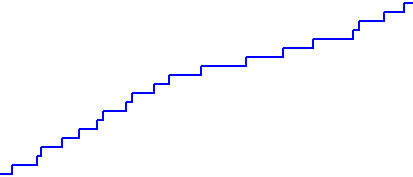
\includegraphics[width=6cm]{Content/Markov/SampleProcessPoisson}
		\end{center}	
	\end{minipage}
	\hfill
	\begin{minipage}{8cm}
		\begin{itemize}
			\item $E(N_t)=\lambda t$
			\item $Var(N_t)=E(N_t^2)-E(N_t)^2=\lambda t$
			\item $\phi(t)=\e^{\lambda t(\e^t-1)}$
			\item $R_N(t,t+s)=\lambda^2 t(t+s)+\lambda t$
			\item $C_N(t_1,t_2)=\lambda\min(t_1,t_2)$
		\end{itemize}
	\end{minipage}
%	\item \todo{Definition 24 auch? (Die sind angeblich gleich wie Definition 23 (Siehe Seite 143))}
	%\item for small $h\geq 0$ we have $P\big(N_h=1\big)=\lambda h +o(h)$ 	\todo{what???}
	%\item for small $h\geq 0$ we have $P\big(N_h\geq 2\big)=o(h)$			\todo{what???}
	\item Given a sequence $\{\tau_n,n\geq 1\}$ of independently and identically distributed exponential random variables.
	
	\begin{minipage}{11.25cm}
	Each having parameter $\lambda$. Define the counting process $\{N_t\geq 0\}$ by the expression:
	$$N_t=max\{n|S_n\leq t \}$$
	
	where $S_n:=\tau_1+\tau_2+\ldots+t_n$ is the time at which the n'th event occurs.
	The counting process $N_t$ is a Poisson process having rate $\lambda>0$.
	$S_n$ is the arrival time of the $n$th event and follows an Erlang$(n,\lambda)$ distribution. It is easy to see that $N_t\geq n \Leftrightarrow S_n\leq t$ (figure right)
	\end{minipage}
	\hfill
	\begin{minipage}{6.25cm}
	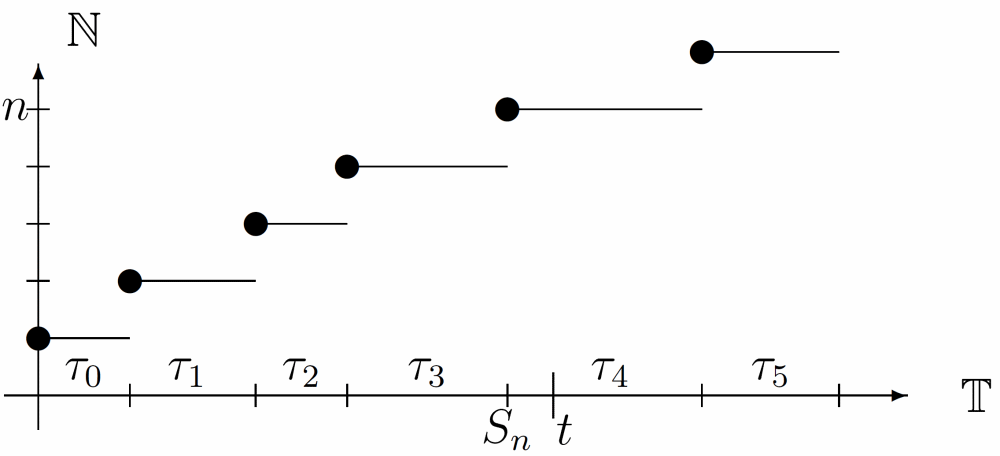
\includegraphics[width=\textwidth]{Content/Markov/erlang}
	\end{minipage}
\end{aufzaehlung}


\begin{minipage}[t]{6.5cm}
\textbf{Generating matrix $G$}:
$$G=\begin{pmatrix}
-\lambda & \lambda & 0 & 0 &\ldots\\
0&-\lambda & \lambda & 0  &\ldots\\
0 & 0&-\lambda & \lambda & \ldots\\
\vdots&\vdots&\vdots&\vdots&\ddots\\
\end{pmatrix}$$

\vspace{0.25cm}

\textbf{Memoryless Expectation $E(\tau)$}:
$$E(\tau|\tau>s)=s+E(\tau)=s+\frac 1\lambda$$

\end{minipage}
\hfill
\begin{minipage}[t]{12.5cm}
\textbf{(Inter)arrival time $\tau$}:
\begin{itemize}
\item (Inter)arrival time: $\tau~Exp(\lambda)$ between two sequentially events:
\item Probability that the (inter)arrival time between two sequentially events is bigger then $s$:\\
 $P(\tau>s)=\int\limits_{s}^{\infty}{\lambda\e^{-\lambda t}dt}=\left[\e^{-\lambda t}\right]_\infty^s=\e^{-\lambda s}$
\item Probability that the (inter)arrival time between two sequentially events is smaller then $s$:\\
 $P(\tau<s)=\int\limits_{0}^{s}{\lambda\e^{-\lambda t}dt}=\left[-\e^{-\lambda t}\right]_0^s=1-\e^{-\lambda s}$
\end{itemize}
\end{minipage}

\renewcommand{\arraystretch}{2}
\begin{tabular}{|l|l|}
	\hline
	\textbf{Two independent Poisson processes with $\lambda_1,\lambda_2$}: & $P(\tau_1 < \tau_2)=\displaystyle\frac{\lambda_1}{\lambda_1+\lambda_2}$ \\
	\textbf{Splitting Poisson process}: & $\lambda_1 = \lambda p \quad \lambda_2 = \lambda (1-p)$\\
	\textbf{Merging two Poisson processes}: & $\lambda = \lambda_1 + \lambda_2$\\
	\hline
\end{tabular}\\
\renewcommand{\arraystretch}{1.0}

\textbf{Examples for some Poisson processes}: 
\begin{itemize}
	\item The total number of persons who enter a particular store
	\item The number of visits of a particular web site
	\item The number of occurrences of earth quakes
	\item The number of occurrences of failure of a given production facility
	\item The number of incoming phone calls in a phone center
	\item The number of electron emission on top of a heated cathode
\end{itemize}

\subsubsection{Birth and death process \skript{145}}

The Poisson process will generalized in a way that allowed the counting process to decrease. Such a process is coined a birth death process. A possible interpretation is the number of clients in a post office where clients enter with exponential arrival times of intensity $\lambda$ and where clients leave the office at an exponential rate $\mu_n$. $n$ is the number of clients in the System.\\

\textbf{Definition of transition rate}: $\nu_{ij}=0 \quad if\quad |j-i|>1$\\

The parameter $\lambda_i:=\nu_{i,i+1}$ for $i\geq 0$ and $\mu_i:=\nu_{i,i-1}$ for $i\geq 1$ are the \textbf{birth rates} and the \textbf{death rates} of the process.\\

Transition probabilities: $p_{01}=1$ and $p_{i,i+1}=1-p_{i,i-1}=\frac{\lambda_i}{\lambda_i+\mu_i}$

\subsubsection{Limiting probabilities \skript{146}}
$$\pi_j=\lim\limits_{n\rightarrow \infty}{p_{ij}(t)}$$
Under ergodic conditions the limit $\pi_j$ exists for all $j \in\{0,1,\ldots\}$ and can be computed by the following \textbf{balance equations} plus probability normalization:
$$\boxed{\underbrace{\pi_j\nu_j}_{\text{outgoing}}=\underbrace{\sum\limits_{i\neq j}{\pi_i \nu_{ij}}}_{\text{incoming}}\quad \text{for all} \quad j\in\{0,1,\ldots \}
\qquad \qquad \sum\limits_{j=0}^{\infty}{\pi_j=1}}$$

\textbf{Interpretation: }\\
Rate at which the process leaves state $j$: $\nu_j\pi_j$\\
Rate at which the process enters state $j$: $\sum\limits_{i\neq j}{\pi_i \nu_{ij}}$

\textbf{Example for Queuing with a single server}\\
\begin{minipage}{10.5cm}
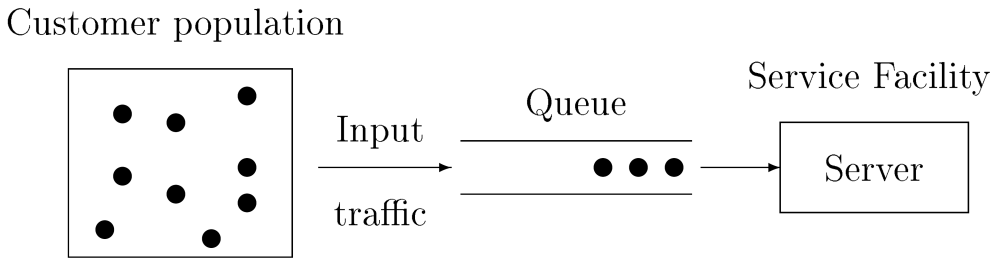
\includegraphics[width=0.8\textwidth]{Content/Markov/Queue.png}
\end{minipage}
\hfill
\begin{minipage}{7.5cm}
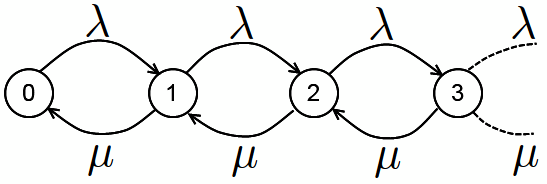
\includegraphics[width=0.8\textwidth]{Content/Markov/queieingGraph.png}
\end{minipage}

\begin{minipage}{5.5cm}
	\textbf{Balance Equation:}
	\begin{align}
		\underbrace{\lambda\pi_0}_{\text{outbound}}			&=\underbrace{\mu\pi_1}_{\text{inbound}}						\nonumber\\[0.25cm]
		(\lambda+\mu)\pi_1		&=\lambda\pi_0+\mu\pi_2	\nonumber\\[0.25cm]
		(\lambda+\mu)\pi_2		&=\lambda\pi_1+\mu\pi_3	\nonumber\\[0.25cm]
		\vdots\qquad			&=\qquad\vdots							\nonumber\\[0.25cm]
		(\lambda+\mu)\pi_{n-1}	&=\lambda\pi_{n-2}+\mu\pi_{n}	\nonumber\\[0.25cm]
		\pi_0+\pi_1+\pi_2&+\ldots+\pi_n=1\nonumber
	\end{align}
\end{minipage}
\hfill
\begin{minipage}{13.5cm}
	\begin{align}
		&\pi_0=\frac{1}{1+\sum\limits_{i=1}^{\infty}{\left(\lambda/\mu\right)^i}}\overset{\frac{\lambda}{\mu}<1}{=}\frac{1}{1+\frac{1}{1-\lambda/\mu}-1}=1-\frac\lambda\mu\nonumber\\[0.25cm]
		&\pi_n=\pi_0\left(\frac{\lambda}{\mu}\right)^n=\left(1-\frac{\lambda}{\mu}\right)\left(\frac\lambda\mu\right)^n\nonumber\\[0.5cm]
		%&\textbf{Total time: }E(X_t)=\todo{???}\nonumber\\[0.5cm]
		&\textbf{Service time: }E(T)=\frac{E(X_t)}{\lambda}\nonumber\\ %\todo{???}\nonumber\\[0.5cm]
		&\textbf{Expected number of clients: }M=\sum\limits_{n=0}^{\infty}{n\pi_n}\nonumber\\
		&\textbf{Use the normalisation: } P\big(n>2\big)=1-\pi_0-\pi_1\nonumber
	\end{align}
\end{minipage} \\

As $\pi_j=\lim\limits_{n\rightarrow \infty}{p_{ij}(t)}$ we can interpret $\pi_j$ as the fraction of time the system 
spends in state $j$ as time goes to infinity. We can also say that $\pi_j$ is the probability to find the system in state $j$.

\vfill



 

